\documentclass[fleqn,compress,utf8,aspectratio=169,t]{beamer}
\usepackage{listings}
\usepackage{hyperref}
\usepackage{xcolor,colortbl}
\usepackage{tabularx}
\usepackage{diagbox}
\usepackage{pifont}
\newcommand{\cmark}{\ding{51}}% checkmark
\newcommand{\xmark}{\ding{55}}% xmark

\usepackage{multirow}

% use LMU theme
\usetheme{LMU}
%\usetheme{CUONG}
%\usetheme{YourOwnTheme}
%remove frame title since it is already inserted in the headline in style/beamerouterthemelmu.sty
%if not use LMU theme, comment out the next 3 lines
\makeatletter
\setbeamertemplate{frametitle}{}
\makeatother


%%%%%%%%%%%%%%%%%%%%%%%%%%%%%%%%%%%%%%%%%%%%%%%%%%%%%%%%%%%%%%%%%%%%%%%%%%%%%%%%
%%                                  Title Page Data                           %%
%%%%%%%%%%%%%%%%%%%%%%%%%%%%%%%%%%%%%%%%%%%%%%%%%%%%%%%%%%%%%%%%%%%%%%%%%%%%%%%%

% helper command to add multiple authors
\newcommand{\newauthor}[2]{
  \parbox[c]{0.26\textwidth}{
        {\bfseries #1} \\
        {\scriptsize{\href{mailto:#2}{#2}}}
      }
      %{#1}
  }

% Multiple Authors
% If you have multiple authors simply use this command and adjust the width in
% style/beamerinnertheme where the authors are rendered
\author[Authors shown in footer]{
    \newauthor{Author 1}{author1@campus.lmu.de} \and 
    \newauthor{Author 2}{mnm-team.org/$\sim$author2}
}

% Single Author
%\author[Vor- Nachname shown in footer]{Vor- Nachname}

%\institute[LMU]{LMU M\"unchen, MNM Team\\\texttt{http://www.nm.ifi.lmu.de/}}
%\institute[LMU]{Ludwig-Maximilians-Universit\"at M\"unchen, MNM-Team}%\\\texttt{http://www.nm.ifi.lmu.de/}}
\institute[LMU]{Aufgabensteller: Prof. Dr. Dieter Kranzlmüller\\
                Betreuer 1:\hspace{5ex} 1. Supervisor \\ 
		Betreuer 2:\hspace{5ex} 2. Supervisor
}

\date[\today]{\today}
%\date[\today]{June 13, 2022}

%title[short title appear in footer of subsequent slides]{Full title in the title page}
\title[Conflict Detection in Software-Defined Networks]{Conflict Detection in \\Software-Defined Networks}
%\subtitle{Subtitle}


%%%%%%%%%%%%%%%%%%%%%%%%%%%%%%%%%%%%%%%%%%%%%%%%%%%%%%%%%%%%%%%%%%%%%%%%%%%%%%%%
%%                                  Document                                  %%
%%%%%%%%%%%%%%%%%%%%%%%%%%%%%%%%%%%%%%%%%%%%%%%%%%%%%%%%%%%%%%%%%%%%%%%%%%%%%%%%

\begin{document}

\begin{frame}
\titlepage
\end{frame}

%%%%%%%%%%%%%%%%%%%%%%%%%%%%%%%%%%% Overview %%%%%%%%%%%%%%%%%%%%%%%%%%%%%%%%%%%

\part{A - Main}
\section{Introduction}

\begin{frame}{Conflicts in Real Life}
\vspace{-0.5cm}
\begin{center}
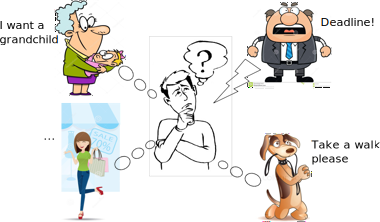
\includegraphics[width=0.88\textwidth]{conflict-real-life}
\end{center}
\end{frame}


\begin{frame}{Conflicts in SDN}
\advance\leftskip+1cm\includegraphics<1>[width=0.8\textwidth]{conflict-sdn1}
\includegraphics<2>[width=0.8\textwidth]{conflict-sdn2}
\includegraphics<3>[width=0.8\textwidth]{conflict-sdn3}

\begin{onlyenv}<4>
\begin{columns}[c]
\column{0.1\textwidth}
\column{0.5\textwidth}
\vspace{1cm}

\textbf{Possible consequences:} 
\begin{itemize}
\item Application's goals are not fulfilled
\item Unexpected, unreliable network behaviour
\end{itemize}
$\textcolor{lmu@hyperlink}{\Rightarrow}$ Conflicts need to be detected and resolved
\column{0.5\textwidth}
\vspace{1cm}
\noindent
\includegraphics[width=\textwidth]{conflict-sdn3}
\column{0.2\textwidth}
\end{columns}
\end{onlyenv}
\end{frame}


\begin{frame}{Conflict Definition}
\vspace{0.5cm}
\begin{center}
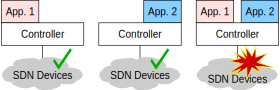
\includegraphics[width=0.7\textwidth]{conflict-definition}
\end{center}
\end{frame}


%\begin{frame}{Goal}
% Goal of this work
%\end{frame}


\begin{frame}{Research Questions}
\vspace{-0.2cm}
\begin{enumerate}
\item<1-> What is a suitable method to research conflicts in SDN? 
\item<1-> How can conflicts between control applications be classified\\ based on their rules (conflict classification)? 
\item<2-> How many conflicts exist in a given rule set (conflict detection)?
\begin{enumerate}
\item Which rules cause conflicts?
\item To which class does each detected conflict belong?
\end{enumerate}

\vspace{0.4cm}

\advance\leftskip+0.7cm
\includegraphics<2>[height=0.45\textheight]{cdinout_highlighted}
\includegraphics<3>[height=0.45\textheight]{cdinout_highlighted_next}
\end{enumerate}

\end{frame}


\section{Related Work}

\begin{frame}{State-of-the-art}
\begin{itemize}
\item Related work 1
\item Related work 2
\item \ldots
\end{itemize}
\end{frame}


\section{Approach}

\begin{frame}{Approach}
\begin{enumerate}
\item Analytical approach 
\item Experimental approach
\end{enumerate}
\end{frame}


\subsection{Experimental approach}

\begin{frame}{Space for Experiments}

\begin{columns}[T]
\column{0.6\textwidth}
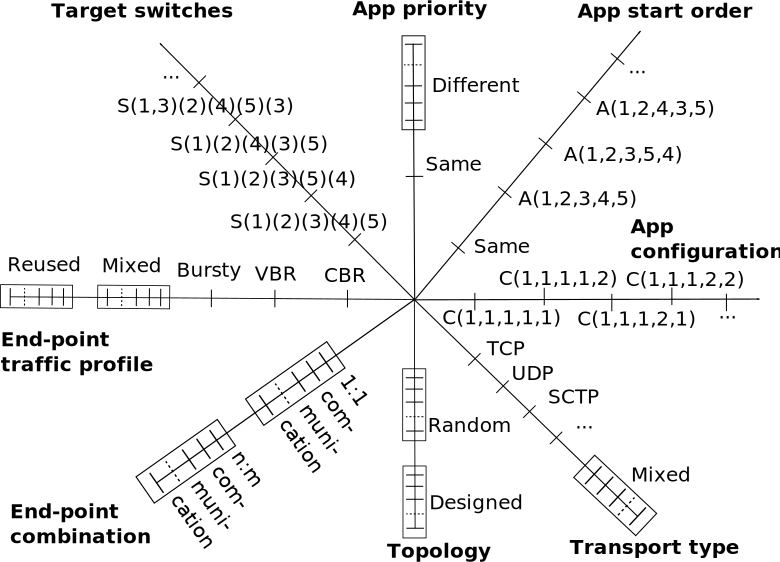
\includegraphics[width=\textwidth]{parameter-space}

\column{0.45\textwidth}
\vspace{7ex}

\begin{onlyenv}<1>
Control applications: 
\begin{itemize}
\item Shortest Path First Routing (SPF)
\item End-point Load Balancer (EpLB)
\item Path Load Balancer (PLB)
\item Firewall (FW)
\item \ldots
\end{itemize}
\end{onlyenv}
\begin{onlyenv}<2>
The number of experiments is immense \\[8pt]
$\textcolor{lmu@hyperlink}{\Rightarrow}$ \textbf{restrict the space size and automate experiments}
\end{onlyenv}
\end{columns}
\end{frame}

\subsection{Methodology for experiments}

\begin{frame}{Methodology for Experiments}
\vspace{-0.3cm}
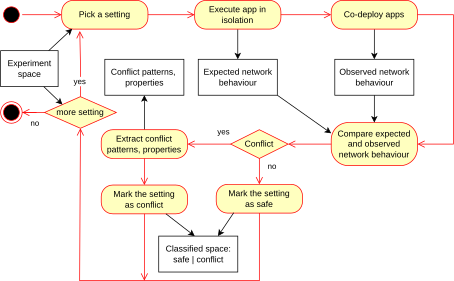
\includegraphics[height=\textheight]{methodology-exp}
\end{frame}


\subsection{Explored subspaces}

\begin{frame}{Explored Subspaces}
\begin{columns}[T]
\column{0.05\textwidth}
\column{0.5\textwidth}
\vspace{0.2cm}
\begin{tabular}{|l|c|}
%\hline
%\textbf{Category} & \textbf{Value} \\
\hline
\# Topologies & 12 \\
\hline
\# Applications & 14  \\
\hline
App. configuration & 1 $\rightarrow$ 5  \\
\hline
App. start order & same and different \\
\hline
App. priority & same and different \\
\hline
Target switches & 1 $\rightarrow$ all \\
\hline
Ep. Traffic Profile & CBR and VBR  \\
\hline
EP. Combination & unicast, multicast \\
\hline
Transport type & TCP, UDP  \\
\hline
\# Experiments & 11,772 \\
\hline
\end{tabular}

\column{0.5\textwidth}
\vspace{0.5cm}
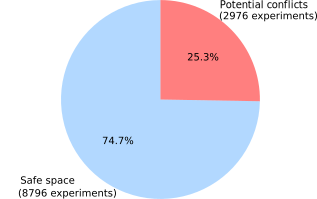
\includegraphics[width=\textwidth]{pie_exp}
\column{0.05\textwidth}
\end{columns}
\vspace{0.3cm}
\scriptsize{Dataset is available at \\https://github.com/mnm-team/sdn-conflicts}
\end{frame}


\section{Multi-property set}

\begin{frame}{Comparing Multi-Property Sets using $\cdot r$}
\vspace{-0.3cm}
\advance\leftskip+1cm 
\includegraphics<1>[height=\textheight]{multi_property_set_comparison_1}
\includegraphics<2>[height=\textheight]{multi_property_set_comparison_2}
\includegraphics<3>[height=\textheight]{multi_property_set_comparison_3}
\includegraphics<4>[height=\textheight]{multi_property_set_comparison_4}
\end{frame}


\section{Prototype}

\begin{frame}{Conflict Detection Prototype}
\vspace{-0.3cm}
\advance\leftskip+1.5cm 
\includegraphics<1>[height=\textheight]{cd_communication}
\includegraphics<2>[height=\textheight]{cd_communication_zoom}
\end{frame}


\section{Evaluation}

\begin{frame}{Detected Results in Designed Cases}

Rules are deployed with known conflicts

Conflicts detected by the prototype are then controlled manually\\[12pt]

Results for both MWN and Stanford topologies:\\[4pt]

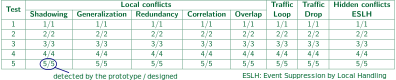
\includegraphics[width=1.05\textwidth]{evares-designed}

\vspace{0.3cm}

$\textcolor{lmu@hyperlink}{\Rightarrow}$ All conflicts are precisely identified

\end{frame}


\section{Conclusions}

\begin{frame}{Conclusions}
\vspace{-0.3cm}
\includegraphics<1>[height=\textheight]{conclusion_rq} %research questions
\includegraphics<2>[height=\textheight]{conclusion}
\end{frame}


\section{Prospects}

\begin{frame}{Prospects}
\vspace{0.3cm}

\begin{itemize}
\item Future work 1
\item Future work 2
\item \ldots
\end{itemize}
\end{frame}

\part{B - Backup}

\begin{frame}[noframenumbering]{Backup}
\end{frame}


\section{Software-Defined Networks}
\begin{frame}[noframenumbering]{Traditional Networks and SDN}
\vspace{-0.3cm}
\includegraphics<1>[height=\textheight]{traditionalnetwork}
\includegraphics<2>[height=\textheight]{traditionalnetworkvssdn}
\end{frame}


\section{Multi-Property Set}
\begin{frame}{Multi-Property Set}
\begin{columns}[T]
\column{0.65\textwidth}
\vspace{0.2cm}

$A$ = a set of flowers having \textbf{five petals}

$B$ = a set of flowers with \textbf{red color}

$C$ = a set of flowers being \textbf{scentless}

\vspace{0.5cm}

\begin{onlyenv}<1->
\underline{Question}: $\textcolor{lmu@hyperlink}{S_{ABC}}$ = a set of flowers having \textbf{five petals,\\ 
                                    \hspace{14ex} red color} and being \textbf{scentless} = ?

\end{onlyenv}
\begin{onlyenv}<2->
\vspace{0.3cm}

\underline{Answer}: \colorbox{green!20}{$\textcolor{lmu@hyperlink}{S_{ABC} = A \cap B \cap C}$}
\end{onlyenv}
\begin{onlyenv}<2->
\vspace{0.3cm}

\textbf{Match fields of SDN rules are multi-property sets}, e.g.,\\
match=\{ip\_src=192.168.1.1, ip\_dst=192.168.1.2,\\ 
       \hspace{8ex} ip\_proto=tcp, tcp\_dst=80\}
\end{onlyenv}

\column{0.4\textwidth}
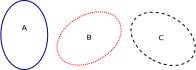
\includegraphics[width=\textwidth]{set_ABC_single}

\vspace{0.3cm}

\includegraphics<2->[width=0.9\textwidth]{set_ABC_multi}

\end{columns}

\end{frame}


\section{Matchmap, actmap}

\begin{frame}{Normalizing SDN Rules by \emph{Matchmap, Actmap}}
\underline{Problem}: diverse expressions of the match and action components of SDN rules complicate their automatic comparison based on multi-property set and $\cdot r$, e.g.,\\[4pt]
rule 1's match: \textit{\{\colorbox{yellow!20}{ip\_src=192.168.1.1}, \colorbox{blue!20}{tcp\_dst=80}\}}\\[4pt]
rule 2's match: \textit{\{\colorbox{pink!20}{ip\_dst=192.168.1.2}\}} \\[8pt]

\begin{onlyenv}<2>
\underline{Solution}: normalizing the match and action components via a common template to obtain their uniform \textbf{matchmap} and \textbf{actmap}, e.g.,\\[4pt]

\begin{center}
\begin{tabular}{|c|c|c|}
\hline
\cellcolor{yellow!20}ip\_src & \cellcolor{pink!20}ip\_dst & \cellcolor{blue!20}tcp\_dst\\
\hline
\end{tabular}
\end{center}

rule 1's \textbf{matchmap}: \textit{\{\colorbox{yellow!20}{ip\_src=192.168.1.1},     \colorbox{pink!20}{ip\_dst=any},\hspace{7ex} \colorbox{blue!20}{tcp\_dst=80}\}}\\[4pt]
rule 2's \textbf{matchmap}: \textit{\{\colorbox{yellow!20}{ip\_src=any}, \hspace{7ex}\colorbox{pink!20}{ip\_dst=192.168.1.2},     \colorbox{blue!20}{tcp\_dst=any}\}}
\end{onlyenv}

\end{frame}


\section{Evaluation}
\begin{frame}{Results in Randomly Checking Cases (MWN)}

The number of conflicts is unknown in advance

Random conflict samples from those identified by the detector are controlled manually

\vspace{0.3cm}

\resizebox{\textwidth}{!}{
\begin{tabular}{|c|c|c|c|c|c|c|c|c|c|c|}
\hline
\multirow{2}{2em}{\textbf{Test}}&\textbf{App} &\textbf{\#} &\multicolumn{5}{c|}{\textbf{Local conflicts}}&\textbf{Traffic}&\textbf{Traffic}&\textbf{HC} \\
\cline{4-8}
  &\textbf{Priority} &\textbf{rules} &\textbf{Sha}&\textbf{Gen}&\textbf{Red}	&\textbf{Cor}&\textbf{Ove}&\textbf{Loop}&\textbf{Drop}&\textbf{ESLH}\\
\hline
1 	& (2,2,2,2) & 790	&0/0/0		&0/0/0		&0/0/0		&27/10/10	&0/0/0		&0/0/0	&0/0/0	&60/10/10 	\\ 
\hline  
2 	& (2,2,3,4) & 803	&0/0/0		&0/0/0		&0/0/0		&26/10/10	&0/0/0		&0/0/0	&0/0/0	&60/10/10 	\\ 
\hline  
3 	& (3,2,2,3) & 816	&0/0/0		&0/0/0		&0/0/0		&27/10/10 	&0/0/0		&0/0/0	&0/0/0	&60/10/10 	\\ 
\hline  
4 	& (3,5,2,4) & 789	&0/0/0		&0/0/0		&0/0/0		&25/10/10	&0/0/0		&0/0/0	&0/0/0	&59/10/10 	\\ 
\hline  
5 	& (5,4,3,2) & 791	&0/0/0		&0/0/0		&0/0/0		&24/10/10 	&0/0/0		&0/0/0	&0/0/0	&60/10/10 	\\ 
\hline
\end{tabular}
}
\vspace{0.1cm}

{\scriptsize{
Each cell shows \textit{the number of conflicts detected by the prototype/ the number of conflicts selected randomly to control/ the number of correct conflicts confirmed based on the manual control}

Sha: Shadowing, Gen: Generalization, Red: Redundancy, Cor: Correlation, Ove: Overlap\\[-1ex]
HC ESLH: hidden conflict class Event Suppression by Local Handling.
}}

\vspace{0.3cm}

$\textcolor{lmu@hyperlink}{\Rightarrow}$ All randomly checking conflicts are correct

\end{frame}




%\input{todo}

%hidden frame for references
\begin{frame}<presentation:0>[noframenumbering]
\nocite{han99}
\bibliographystyle{IEEEtran}
\bibliography{paper}
\end{frame}

\end{document}
